\documentclass[a4paper, 12pt, conference]{IEEEtran}
\special{papersize=210mm,297mm} % Fix compatibility issues. A4 dimensions hard coded.
\usepackage[a4paper, top=0.8in, bottom=0.8in, left=0.6in, right=0.6in]{geometry}
\usepackage[utf8]{inputenc}
\usepackage[pdftex]{color, graphicx}
\usepackage[official]{eurosym}
\usepackage{fancyhdr}
\usepackage{amsfonts}
\usepackage{amsmath}
\usepackage{amsthm}
\usepackage{amssymb}
\usepackage{tabularx, caption}
\usepackage{setspace}
\usepackage{soul} % Text highlighting
\usepackage{type1cm} % Scalable Computer Modern font support
\usepackage{verbatim}
\usepackage{hyperref} % Support for PDF Hyper References and links
\usepackage{lastpage} % To get number of pages
\usepackage{listings} % To include code blocks
\usepackage{color}
\usepackage[acronym]{glossaries}

\def\arraystretch{1.4}

\newcommand{\upsc}[1]{\textsc{#1}}
\loadglsentries{acronyms}  
\makeglossaries

\newcommand{\todo}[1]{}
\renewcommand{\todo}[1]{{\color{blue} TODO:  {#1}}}

\def \FIXME {{\parindent -60px \sethlcolor{red} \color{white} \texthl{\textbf{FIXME}} \sethlcolor{yellow} \hskip 5px}}
\def \redhl #1{\sethlcolor{red} {\color{yellow} \textbf{\texthl{#1}}} \sethlcolor{yellow}}
\def \sitat #1{\textsuperscript{\cite{#1}}}
\def \const #1{\penalty 100 \hbox{\texttt{#1}}}
\newcommand{\HRule}{\rule{\linewidth}{0.2mm}}



\hypersetup{
colorlinks,%
citecolor=black,%
filecolor=black,%
linkcolor=black,%
urlcolor=black%
}

\setlength{\headheight}{14pt}

\ifCLASSINFOpdf

\else

\fi

\hyphenation{op-tical net-works semi-conduc-tor}
\def \thetitle {Awesome graph database benchmark shit}
\def \thesubtitle {}
\def \theauthor {Helge Hoff, Kim Hartvedt Andreassen, Jon Foss Mikalsen}
\def \thecocks{helge.hoff@uit.no}

%\pagestyle{fancy}
\pagestyle{fancyplain} % options: empty , plain , fancy
\renewcommand{\headrulewidth}{1pt} % customise the layout...
\renewcommand{\footrulewidth}{0pt}
\lhead{\fancyplain{}{\thetitle{} -- \thesubtitle{}}}
\lfoot{}\cfoot{Page {\thepage} of \pageref{LastPage}}\rfoot{}
\begin{document}
\title{\thetitle}
\author{\theauthor}

\maketitle
\pagestyle{fancy}
%ABSTRACT
%\begin{abstract}
%When written in 
%\end{abstract}
 
\IEEEpeerreviewmaketitle

\section{Introduction}

\section{Background}
Social network applications are becoming increasingly popular, and traditional SQL databases are not well-suited to store large social networks with relationships between users.
Representing relationships in SQL databases often results in inefficient table joins, degrading performance significantly.
 
\todo{Use citation, explain neo4j scaling(index-free-adjacency)}
\cite{neo_scale}
\section{Data Migration}

This section describes our experience with data migration from an existing relational database into a Neo4j graph database. 
We use a subset of an implemented MySQL data model from one of our previous projects; an application called \textit{ShareDrive}.

\subsection{Relational Model} 
ShareDrive is social network application for sharing files amongst friends. 
A registered ShareDrive user can share a local directory on their computer through a client-side application. 
The web application will then synchronize metadata of the directory's containing files with a remote database, allowing for the users friends to browse the content through the web application and download the files directly from the user (peer-to-peer). 
Through the web application, users can (amongst other things) add new friends, post messages and search for files their friends are sharing.

The underlying \gls{rdbms} of ShareDrive is MySQL, its schema consisting of ten tables describing users, roles, friends, logs and so on.
Our data migration experiment is applied to a subset of this schema, which represents the core functionality of ShareDrive. Figure \ref{fig:sql_db} shows the data model of this subset as represented in the relational database.

\begin{figure}[h]
	\centering
	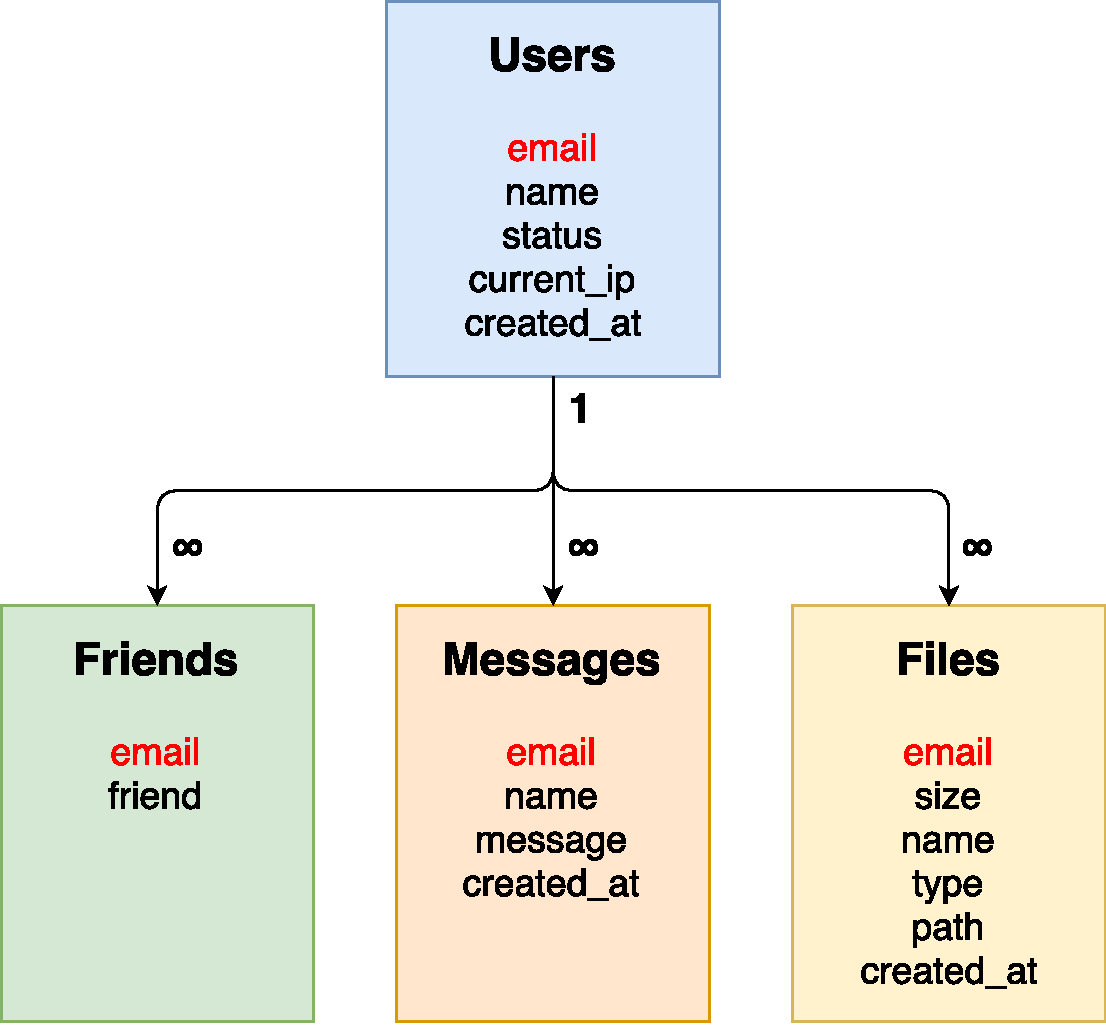
\includegraphics[scale=0.45]{sql.pdf}
	\caption{Subset of ShareDrive's relational model}
	\label{fig:sql_db}
\end{figure}

A users e-mail address is the primary key of all underlying tables, as this is unique for each user. 
Each table contains columns describing properties or relationships of its object, such as the friends of a user or the size of a file he is sharing.
Typical queries such as “find all movies shared by my friends” or “find a message posted by Alice the last hour” requires nested join operations between tables in order to produce the correct results. 
Though forming these queries aren't necessarily difficult, these tables can be arbitrarily large, which may result in poor performance when joining multiple tables. 
Using a sequential data model often results in duplicate data in order to properly connect related objects.
\subsection{Graph model}
In order to create a subset of ShareDrive's data model as a graph database, we implemented a small API. 
Using this interface, constructed of Cypher queries, we can add nodes and their properties into our graph database. 
Figure \ref{fig:graph_db} shows an example graph of a database consisting of three users, their relationship, files they are sharing and messages they've posted.

\begin{figure}[h]
	\centering
	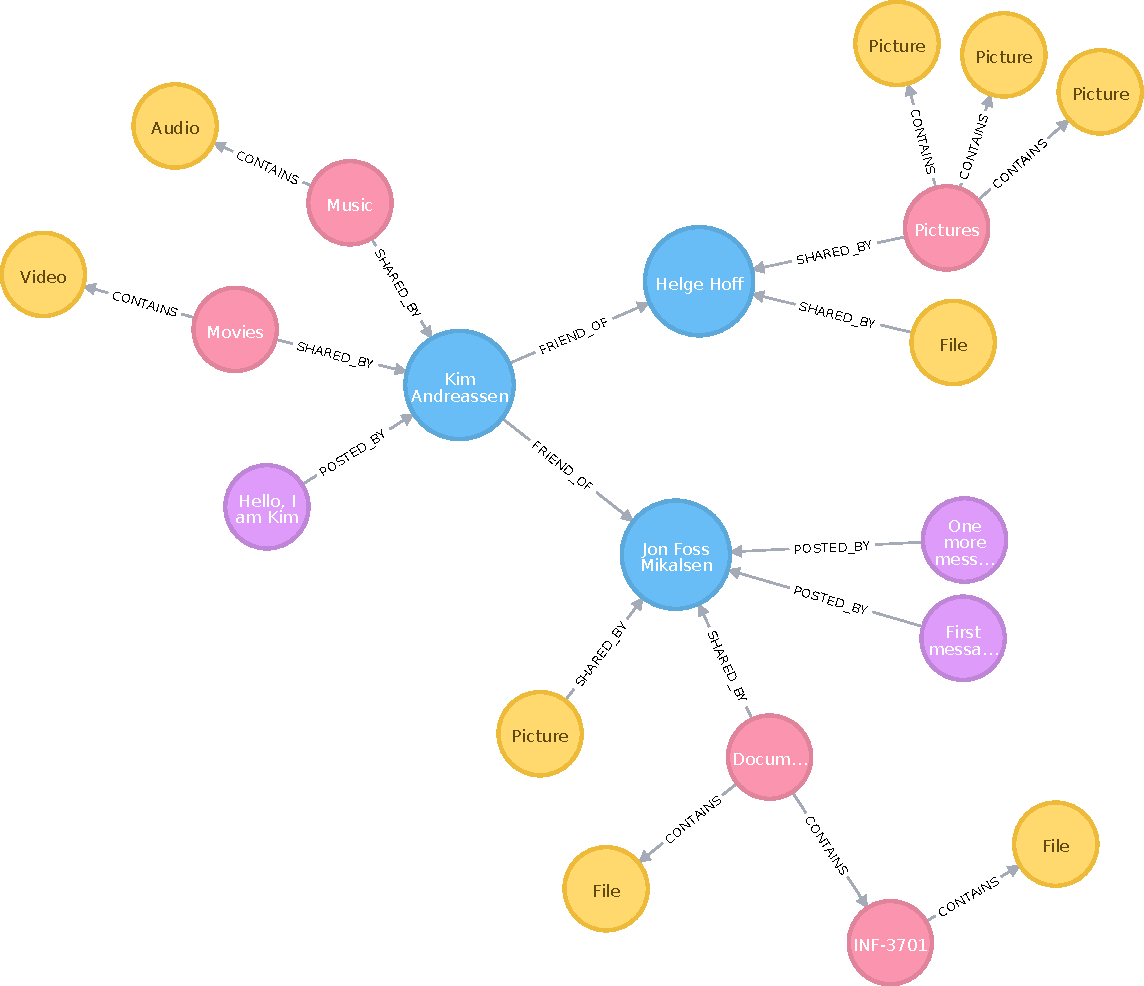
\includegraphics[scale=0.45]{graph.pdf}
	\caption{Subset of ShareDrive as a graph model}
	\label{fig:graph_db}
\end{figure}

The blue nodes in the figure represent users, which are connected to each other through a \textit{FRIEND\_OF} relationship. 
As a friendship is mutual between users of ShareDrive we implicate this relationship to be bidirectional, even though its expressed as a directed relation in Neo4j. 
Red nodes represent folders and yellow nodes represent files. 
Files or folders that reside in the users root share folder are connected by a \textit{SHARED\_BY} relationship to the user node. 
Nested files and sub-folders are further connected by a \textit{CONTAINS} relationship with their parent folder. 
The purple nodes represent messages a user have posted on the message board, connected to a user with a \textit{POSTED\_BY} relationship.

Each node contains relevant properties for its type. 
These properties were originally represented as columns in the sequential database (see Figure \ref{fig:sql_db}). 
In example, a \textit{File} node contains the properties file name, size, file type, its absolute path and a timestamp of its creation.
\subsection{Queries}
Having successfully migrated a subset of the ShareDrive database, we wish to investigate its applicability by re-writing some commonly used SQL queries in the ShareDrive application into Cypher queries. 
These queries are essentially used by the web application in order to retrieve and display data.

Listing \ref{lst:sql_query} shows a sample SQL query of how a user can find all pictures shared by his friends with a name containing the word \textit{cat}.

\lstset{
	keywordstyle=\color{blue}
}

\begin{figure*}
\begin{lstlisting}[caption=SQL Query, language=sql, basicstyle=\small, xleftmargin=.1\textwidth, xrightmargin=.1\textwidth, frame=tb, label={lst:sql_query}]
SELECT (Records.type) FROM Records 
INNER JOIN Users 
ON Users.email = records.email 
WHERE (Records.name LIKE "cat%" OR 
       Records.name LIKE "%cat%") 
AND Records.email
IN (SELECT Friends.friend FROM Friends 
    WHERE Friends.email = "user@mail.com") 
AND Records.type = 'Picture'
\end{lstlisting}
\end{figure*}
Here is an equivalent query using Cypher:
\begin{figure*}
\begin{lstlisting}[caption=Cypher Query , language=sql, basicstyle=\small,
xleftmargin=.1\textwidth, xrightmargin=.1\textwidth, frame=tb, morekeywords={RETURN}, label={lst:cypher_query}]
MATCH (u:User {email: "user@mail.com"})-[:FRIEND_OF]-(friends)
MATCH (friends)-[:SHARED_BY]-(folder)-[:CONTAINS*0..]-(files:File)
WHERE files.type = "Picture" AND files.name =~ ".*cat.*"
RETURN files as name
\end{lstlisting}
\end{figure*}
Having experience with SQL beforehand, we find that Cypher is not only similar in many ways, but easier to read, write and understand. 
On complex queries that involves a series of join operations and additional attribute look-ups, SQL becomes less readable. 
Because the data resides in tables, programmers must always have a clear understanding of the schema layout when writing these queries. 
In Cypher, the query is formed in a consecutive manner as the programmer can naturally write queries continuously by keeping track of relationships along the way. This results in a more intuitive and simple process of forming queries.

\subsection{Comparison of modeling data}
In our experience, Neo4j proves to be most suitable for modeling ShareDrive's data. The graph data model is more intuitive and straightforward, making it easy to represent connected data and semi-structured data, as found in ShareDrive. 
We more or less store the data as it is in the real world; small, normalized, yet richly connected. 
The relational model is by no means useless, as it's proven to be adequate in supporting ShareDrive's core functionality for some time now. 
The graph model provides the developer with a simpler and more elegant solution for modeling data that are inherently related.

The data model described in Figure \ref{fig:sql_db} illustrates how the relational model may be confusing when dealing with related data. 
The \textit{Messages} table contains a \textit{name} column, in order to display the name of the poster of a message with one simple query to the table. 
This extra column is redundant, as the name is easily found by a simple lookup in the \textit{Users} table, but will add additional complexity to the query. 
We might say that the data is poorly structured by the programmer, but it illustrates the shortcuts we are prone to make when having relationships between tables in the relational data model.

Using graphs to model our data provides a cleaner structure, avoiding redundant tables and data entries. 
The friend-relationship is a good example of this. 
In the relational database, friend-relationships are stored as a two-way relationship. 
This results in two table entries (one for each direction) per friend-relationship, causing data redundancy. 
In the graph database, we form one relationship between the User nodes and are able to traverse it both ways, greatly simplifying our design.

Connecting related data in relational databases can be a tedious and complex task. ShareDrive's data model forms a one-to-many relationship from the a user to its contained data, which allows for simple join operations between tables to fetch queried data. 
Problems occur when data are expressed by a many-to-many relationship. 
This will require additional link-tables containing foreign keys from related data in other tables, just to do a simple join operation. 
In the graph model, many-to-many relationships are no more complex than a one-to-many relationship, as we just add more edges between already existing nodes.

\section{Benchmark}
The benchmark consisted of finding friendship relations between users within a social network.
Finding friends of a user, friends of friends and so on, for each increment the result set increases exponentially, as shown in figure one.
Such queries are typical for real-time social network applications, such as Facebook or Twitter. These queries are latency sensitive, making performance vital for the user experience.
Figure one shows a friends of friends query. It's clear that for each depth increment the involved data set increases exponentially.
\begin{figure}[h]
	\centering
	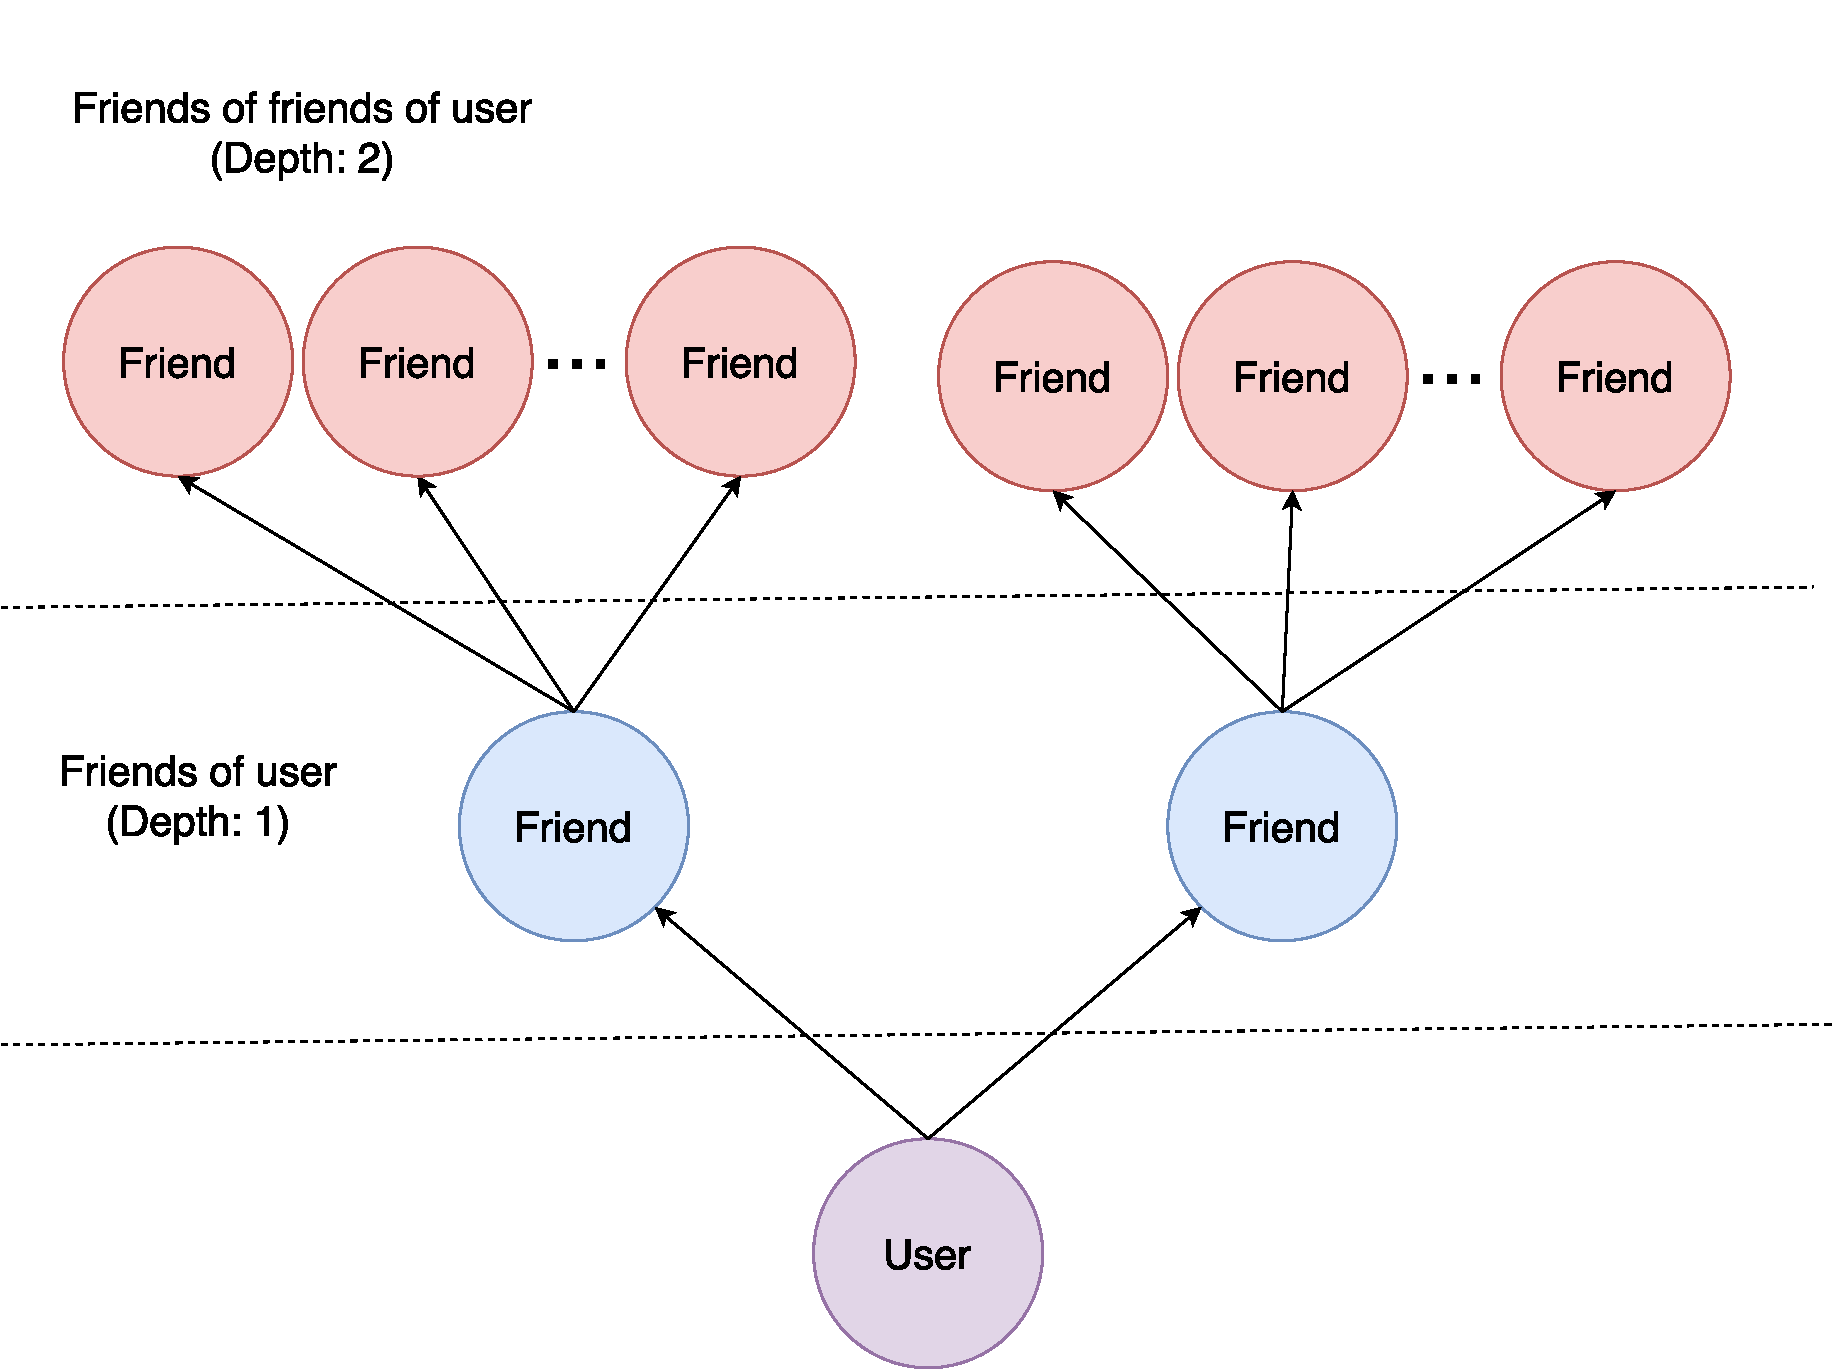
\includegraphics[scale=0.28]{friends.pdf}
	\caption{Query model for multi-level friendship queries.}
	\label{fig:friend_query}
\end{figure}
\subsection{Experimental setup}
To conduct the experiment we used a dataset from Facebook, containing users and their social circles.
The dataset includes several features describing anonymous Facebook users. However, for our experiment only friendships between users were included.
Our test environment is as follows: 
\begin{itemize}
	\item Processor: Intel® Core™ i7-4500U CPU @ 1.80GHz.
	\item 8GB of memory. 
	\item Neo4j version: 3.1.2
	\item SQL database: MySQL 5.7.17
	\item Operating system: Ubuntu 16.04
\end{itemize}
Friendships on Facebook have to be mutual, and only requires a one-way relationship. For query simplicity, however, we represent them as a two-way relationships in the SQL database.
Neither the SQL nor Neo4j database have indexes.
\subsection{Performance}
The queries performed are intended for real-time computation.
Hence, performance has to be within a reasonable time-frame to be considered suitable for applications.
As depicted in table one, Neo4j outperforms MySQL by an order of magnitude, which becomes evident as the depth increases, and thereby relational complexity.
Neo4j has acceptable performance for real-time computation for all levels of depth, while MySQL diminishes at depth three.
For each depth level, MySQL has to perform more costly join operations on increasingly large tables.
As mentioned, the result set increases exponentially for each increment of depth, and due to Neo4j's index-free adjacency its performance is not affected in the same manner as MySQL.

Traversing a relationship between two nodes in a Neo4j graph remains constant when the dataset increases, while SQL database lookups and joins becomes more expensive.
It has been shown before \cite{comparison} that Neo4j has performance advantages over MySQL, or in general the relational model approach.
These advantages were mainly observed in queries involving traversals of relationships, which in the relational model approach requires expensive table joins.
Additionally, relational models often represent relationships by duplicating data in supplementary tables, often referred to as link tables.
A link table has the sole purpose of acting as a "link" between two or more tables, only being utilized during join operations.
Graph databases avoids this by representing relationships within the graph. 
    
It's clear that MySQL lacks the performance required by certain online systems.
A Facebook user would not find it acceptable to wait 94 seconds for a search query to finish.
Even if MySQL performs acceptable from depth one through three, if the dataset was increased, MySQL would fall off earlier due to the increasingly expensive table joins. 
Although, one could argue that searching for such remote friends is rare, and maybe not a valid use case at all.
Even if we substitute the social network for a different domain such as bio-informatics, stock markets, music or data management, we would experience similar benefits in performance and ease of data modeling \cite{graph_book}.
   
\begin{table}[t]
	\centering
	\begin{tabular}{c|c|c}
		\textbf{Depth} & \textbf{Neo4j} (s) & \textbf{MySQL} (s) \\ \hline
		1 & 0.0238 & 0.0563 \\ \hline
		2 & 0.0366 & 0.147 \\ \hline
		3 & 0.143 & 3.136 \\ \hline
		4 & 0.378 & 94.001 \\
	\end{tabular}
	\caption{Performance comparison of multi-level friendship queries between Neo4j and MySQL. Query times are shown in seconds.}
\end{table}

\section{Experience}
Neo4j's graph model has better capabilities to facilitate modeling of complex relational data than that of relational databases, both in terms of 
scalability and flexibility.
Constructing graph databases is intuitive and not constrained by a defined schema.
Instead, it's constantly changing as new relationships are added.

Relational databases were initially designed to codify paper and tabular structures, which they do exceedingly well, but struggle to model relationships.
Ironically, relational databases deals poorly with relationships \cite{graph_book}.
Relationships only exist at modeling time and is not an inherent property of the database.
As the overall dataset becomes more complex and less uniform, the relational model is impeded with large join tables, barely populated rows and extensive null-checking logic. 
Increased connectedness results in additional joins that affects performance, making it difficult for an existing database to adapt in response to business requirements.

Changes to a schema in a relation database requires migration and extensive care when foreign or primary keys are altered.
As a result, maintenance becomes a tedious task and requires users to have extensive knowledge of their data model and SQL.
Graph databases excels at continuous changes, as new relationships are added without requiring frequent migrations.
This relieves users of the dreary task of frequently updating a schema and migrating the entire database for minor changes.

In our experience, Neo4j excels where the relation model struggle. 
To accommodate relationships between data, the relational model requires additional elements to their model design, as opposed to Neo4j where they are first-class citizens.
Graph databases are "white-board friendly", as they naturally fit the way we tend to organize data when drawn on a white-board. By using boxes and circles as components, and lines or arrows to represent relationships, the sketches become quite similar to the data model later implemented within the database.

Neo4j provides a HTTP-API for users to easily access data in a programmatic manner.  
Data can be imported to Neo4j from an existing relational database, by creating a CSV dump file from the existing database and importing it with Cypher's LOAD CSV tool.
From our experience, both the HTTP-API and database imports in Neo4j are intuitive and simplistic.
Neo4j also implements a graphical user interface(GUI), providing users with the ability to observe changes and additions applied to a graph.
For new users, the GUI is a great tool to understand the semantics of how Neo4j functions.
        

\section{Conclusion}


%%% BIBLOGRAPHY

\newpage

\bibliographystyle{ieeetr}
\bibliography{sources}

\end{document}







